\section{Numerical comparisons at a fixed pull budget}
\label{sec:experiments}

We examine the cost of maintaining reliable reports at an actual sampling
budget, including settings in which the conservative checkpoint construction
is impractical. These comparisons assess finite-budget behavior. The four
environments are not the separated family used for the two-endpoint theorem,
and the simulations do not test its asymptotic rates.

\subsection{Protocol and competing rules}

All rewards are Bernoulli. We fix $T=20{,}000$, $\varepsilon=.30$,
$\eta=.10$, and $\delta=.05$, with eight arms by the end of each run.
There are 160 independent replications per environment. Within a replication,
every method receives the same potential reward stream for each arm; its
$n$th pull of arm $i$ reveals the same $X_{i,n}$. Thus methods share the
underlying observations without being forced to take the same actions.
Arrivals occur before the action, reports follow the observation, and all
methods retain previous observations. The full arrival times, means, seeds,
and policy definitions are saved in a single configuration file.

The first environment has initial means $.65,.50$ and three later batches of
inferior arms, so the benchmark remains constant. The second has four
successive benchmark levels $.45,.70,.90,.98$; some earlier unresolved
membership questions become obsolete when a better arm arrives. The third
introduces six arms at one time, including a new best arm. The fourth ends
arrivals at pull 4037 and leaves nearly 16,000 further pulls for recovery.
Noninitial batches occur 36 pulls after a 100-pull admission grid, so the
short-period baseline is not evaluated only at its most favorable alignment.
No policy is given future arrivals, the means, or the evaluation horizon.

We implement CP-UCB-AA with FIFO service every second pull at two fixed
precisions. The choice $\rho=.04$ satisfies $2\rho<\eta$: on the coverage
event, completing all checkpoints resolves every $\eta$-separated arm.
The choice $\rho=.12$, inherited from the implementation supplied with the
theoretical development, is a coarser engineering setting. Its labels remain
reliable, but it need not resolve every arm counted by the $\eta=.10$ metric.
We report these choices separately. With eight arms their total checkpoint
quotas are 73,083 and 8,123 pulls, respectively. The finer setting therefore
cannot complete all quotas within the chosen budget.

Three comparisons isolate the allocation rule while retaining the coarser
checkpoint report: FIFO service every eighth pull, confidence-driven service
every second pull, and full-history UCB without designated service pulls.
Confidence-driven service samples the widest interval among unresolved arms
and the arm with largest upper endpoint, breaking ties by sample count and
then arrival order. It stops designated service when no report remains
unresolved. A completed checkpoint retains its fixed interval.

We also use the full-prefix confidence report from the theory with three
reward or sampling rules. UCB-prefix admits every arm immediately and uses
the same full-history UCB index as CP-UCB-AA. Growing-MOSS uses the anytime
index
\[
 \widehat\mu_{i,n}
 +\sqrt{\frac{\max\{\log(t/(K_tn)),0\}}{n}},
\]
with infinite index at $n=0$; no minimax property of the fixed-horizon MOSS
algorithm is assumed for this extension. ALL-$\varepsilon$ adaptation uses
the confidence-driven service rule every second pull and UCB otherwise.
It retains all history and can revise positive reports after arrivals.
This is a natural adaptation of confidence-based all-good-arm sampling,
not an implementation of FAREAST or $(\mathrm{ST})^2$.
Finally, Batch100-UCB follows the reviewer's proposed short-admission
comparison: it admits waiting arms at pulls $1,101,201,\ldots$, uses UCB on
the admitted reward-active arms, and retires an arm from reward sampling when
its upper bound falls below the largest active lower bound. It retains all
observations. Its report covers all physically arrived arms, including those
still waiting for admission, whose intervals are $[0,1]$.

Table~\ref{tab:simulation} gives means and Monte Carlo standard errors.
Figure~\ref{fig:cost-area} includes every method; error bars are 1.96 Monte
Carlo standard errors. The released data also contain paired differences,
all unresolved paths, service pulls, and the regret charged to service.
The compiled implementation was checked against the original CP-UCB-AA
\texttt{choose/observe/report} class for 20,000 successive rounds: actions,
service indicators, every available-arm count, and every reported label
agreed at each round.

\input{experiments/results/table_main.tex}

\begin{figure}[t]
\centering
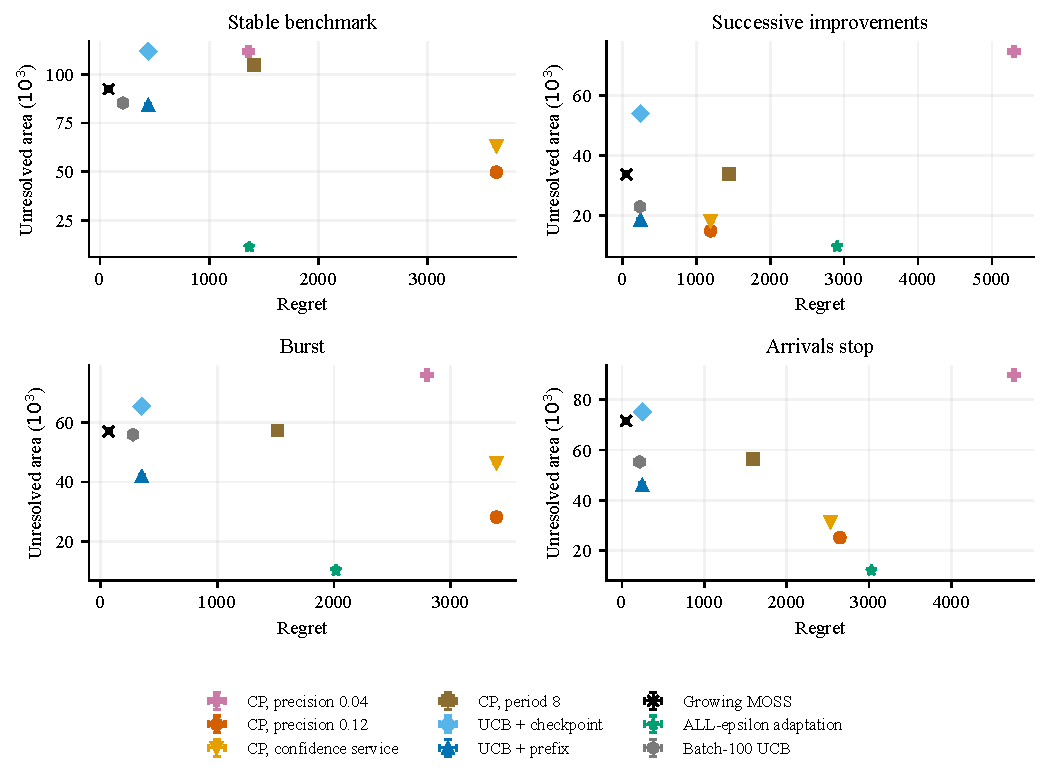
\includegraphics[width=.97\textwidth]{figures/fig_cost_area.pdf}
\caption{Regret and cumulative $\eta$-unresolved area for all nine methods.
Lower values on both axes are preferable. Error bars quantify Monte Carlo
uncertainty, not uncertainty in the theoretical reliability statement.
Neither checkpoint precision nor its allocation variants uniformly dominate
the confidence-based adaptation.}
\label{fig:cost-area}
\end{figure}

\subsection{What the comparisons show}

The finer checkpoint rule leaves between five and eight
$\eta$-unresolved arms on average at the final pull, depending on the
environment. Its unresolved area ranges from 74,820 to 111,784.
This is an observable limitation of the conservative construction, rather
than evidence that arrivals are intrinsically unmanageable at this budget.
The confidence-based adaptation resolves all $\eta$-separated arms by the
end in every replication of these four environments.

The coarser checkpoints reduce area substantially relative to UCB alone,
but can incur much larger regret. Under a stable benchmark, CP-FIFO has
mean regret 3629.9 and area 49,718, compared with 1367.8 and 11,306 for
ALL-$\varepsilon$ adaptation. The paired differences, CP-FIFO minus the
adaptation, are $2262.1$ (standard error $11.7$) for regret and $38{,}411.7$
(standard error $241.9$) for area. The adaptation also improves both
quantities in the burst environment. These comparisons do not support a
general numerical advantage of checkpoint FIFO over a strong
history-retaining identification rule.

In the successive-improvement environment, CP-FIFO instead occupies a
different cost point: regret 1194.7 and area 14,743, compared with 2905.8
and 9525 for the confidence-based adaptation. Here the paired regret
difference is $-1711.0$ (standard error $2.4$), while the area difference is
$5217.7$ (standard error $141.1$). This is consistent with the distinction
between spending pulls to resolve current membership questions and allowing
some questions to be superseded by later arrivals. It is not an estimate
of an optimal Pareto frontier.

Growing-MOSS has the smallest mean regret in all four environments,
between 52.0 and 77.3, while leaving substantially larger unresolved areas.
Low regret therefore provides little evidence of timely set maintenance.
Conversely, the explicit service rules pay for observations of inferior
arms. Reducing service from every second to every eighth pull generally
reduces regret and enlarges unresolved area. Replacing FIFO by the
confidence-driven checkpoint allocation does not uniformly improve either
criterion; allocation and the report's precision both matter.

\begin{figure}[t]
\centering
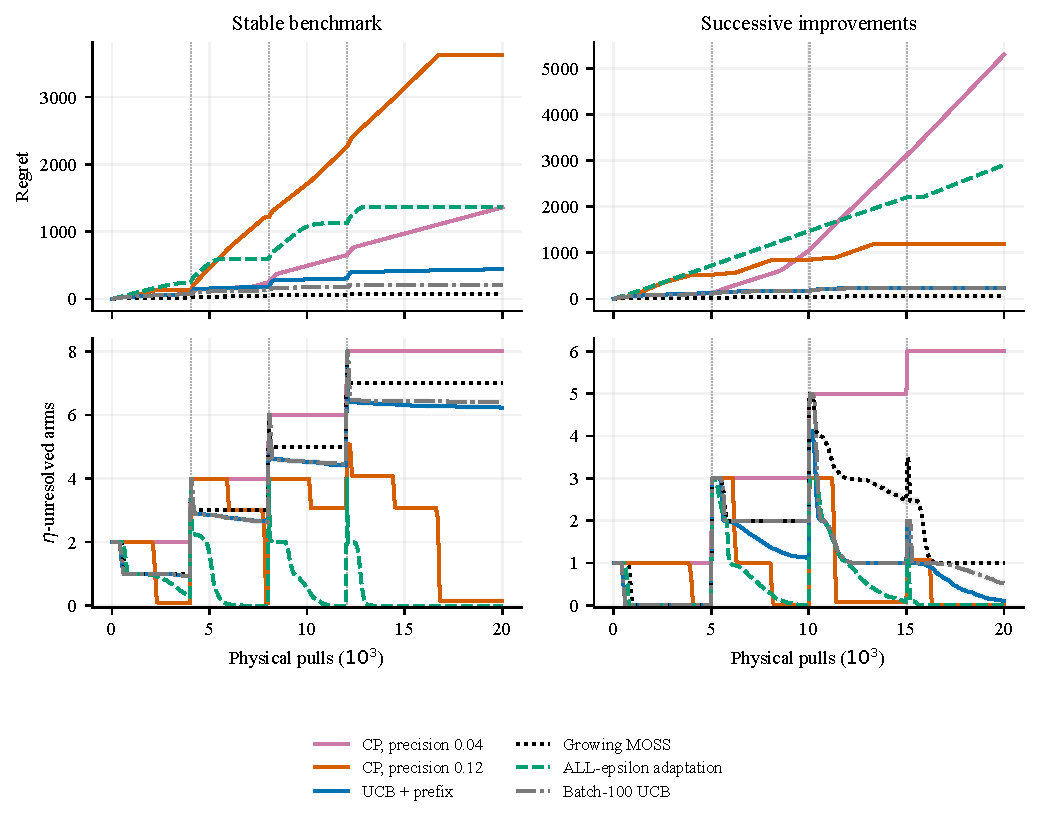
\includegraphics[width=.98\textwidth]{figures/fig_paths_pair1.pdf}
\caption{Mean regret and mean $\eta$-unresolved arm counts at the physical
sampling clock. Bands are 1.96 Monte Carlo standard errors; vertical dotted
lines mark arrivals. Stable and improving benchmarks are shown here;
the other environments appear in the supplement. The main six methods are
displayed; all nine methods and all sampled paths are retained in the released results.}
\label{fig:paths}
\end{figure}

For Batch100-UCB we additionally record the exact decomposition into
within-active regret, admission delay, and loss from previous reward
retirement. Its admission-delay contributions are $0$, $33.92$, $16.00$,
and $22.40$ in the four environments. No historical-retirement deficit
occurred in these runs. The largest discrepancy between total regret and
the sum of the three recorded components was below $3.1\times10^{-12}$.
The corresponding admission and retirement terms are identically zero for
the methods that admit every arm immediately and retain every arm for
reward selection. This accounting avoids attributing every loss outside
within-active learning to arrival delay.

There were no incorrect positive or negative reports in any of the 5760
runs. For one fixed environment and method, zero failures in 160
replications gives a one-sided 95\% upper confidence bound of 0.0186 on
its failure probability. This finite set of diagnostics does not establish
the uniform, all-environment reliability guarantee. Nor do these small
eight-arm experiments validate the asymptotic lower bounds, resolve the
critical logarithmic gap, or establish checkpoint optimality. They show
the practical cost of the conservative quotas and the importance of
comparing retained-history methods under both regret and maintenance
criteria.
